\documentclass[11pt,a4paper]{article}

% --- Packages de mise en page et typographie ---
\usepackage[utf8]{inputenc}
\usepackage[T1]{fontenc}
\usepackage[french]{babel}
\usepackage{lmodern}
\usepackage{geometry}
\geometry{top=2.2cm, bottom=2.2cm, left=2.2cm, right=2.2cm}
\usepackage{setspace}
\setstretch{1.15}

% --- Packages Mathématiques & Symboles ---
\usepackage{amsmath, amsfonts, amssymb, amsthm, bm, mathtools}
\usepackage{physics}

% --- Graphiques, Couleurs & Figures ---
\usepackage{graphicx}
\usepackage{xcolor}
\usepackage{tikz}
\usetikzlibrary{shapes, arrows, positioning, calc, fit, backgrounds, decorations.pathreplacing}
\usepackage{subcaption}
\usepackage{float}
\usepackage{booktabs}
\usepackage{array}
\usepackage{multirow}

% --- Boîtes colorées & Présentation ---
\usepackage[most]{tcolorbox}
\tcbset{
    enhanced,
    colback=gray!5,
    colframe=teal!70!black,
    fonttitle=\bfseries,
    arc=4mm,
    boxrule=1pt,
    left=4mm, right=4mm, top=3mm, bottom=3mm
}

% --- Hyperliens & Navigation ---
\usepackage{hyperref}
\hypersetup{
    colorlinks=true,
    linkcolor=teal!80!black,
    citecolor=blue!70!black,
    urlcolor=cyan!70!black,
    pdfauthor={PRADAS Project Team},
    pdftitle={Rapport Scientifique et Technique PRADAS — YOLOv11 + CrowdHuman + MOT17}
}

% --- Définition des couleurs corporate ---
\definecolor{pradasblue}{RGB}{0, 102, 204}
\definecolor{pradasdark}{RGB}{15, 23, 42}
\definecolor{pradascyan}{RGB}{0, 240, 255}
\definecolor{pradasgreen}{RGB}{16, 185, 129}
\definecolor{pradasamber}{RGB}{245, 158, 11}
\definecolor{pradasred}{RGB}{239, 68, 68}

% =========================================================================
% DOCUMENT PRINCIPAL
% =========================================================================
\begin{document}

% -------------------------------------------------------------------------
% PAGE DE TITRE ACADÉMIQUE
% -------------------------------------------------------------------------
\begin{titlepage}
    \centering
    \vspace*{0.5cm}
    
    {\scshape\LARGE Université des Sciences et de la Technologie\par}
    {\scshape\Large Faculté d'Informatique \& Génie Électrique\par}
    {\large Master S9 — Intelligence Artificielle \& Deep Learning Avancé\par}
    \vspace{1.5cm}
    
    \begin{tcolorbox}[colback=pradasdark, colframe=pradascyan, arc=3mm, width=0.95\textwidth, halign=center]
        \vspace{0.4cm}
        {\Huge \bfseries \color{white} P R A D A S \par}
        \vspace{0.3cm}
        {\Large \bfseries \color{pradascyan} Pedestrian Risk-Aware Driver Assistance System \par}
        \vspace{0.2cm}
        {\color{gray!30} \small Système Embarqué d'Aide à la Conduite Autonome pour la Détection, l'Évaluation de Risque Collision et le Freinage d'Urgence en Temps Réel}
        \vspace{0.4cm}
    \end{tcolorbox}
    
    \vspace{1.2cm}
    
    \textbf{\Large RAPPORT SCIENTIFIQUE, THÉORIQUE ET TECHNIQUE}\par
    \vspace{0.3cm}
    {\large De la Formulation Mathématique de l'Optimisation Profonde à l'Intégration d'un Cockpit Automobile Réactif}
    
    \vspace{2cm}
    
    \begin{minipage}{0.48\textwidth}
        \begin{flushleft} \large
            \emph{Auteur :}\\
            \textbf{Younes Bouderba}\\
            \small Étudiant Ingénieur / Chercheur Master\\
            \small Spécialité Vision par Ordinateur \& IA
        \end{flushleft}
    \end{minipage}
    \hfill
    \begin{minipage}{0.48\textwidth}
        \begin{flushright} \large
            \emph{Projet de Recherche :}\\
            \textbf{PRADAS v2 — 2026}\\
            \small Architecture : YOLOv11s + MiDaS + ByteTrack\\
            \small Datasets : CrowdHuman + MOT17 Joint
        \end{flushright}
    \end{minipage}
    
    \vfill
    
    {\large \today}\par
    \hrulefill\\
    \footnotesize Code Source \& Résultats : \url{https://github.com/younessa04/Pradas}
\end{titlepage}

\newpage
\tableofcontents
\newpage

% -------------------------------------------------------------------------
% RÉSUMÉ EXÉCUTIF
% -------------------------------------------------------------------------
\section*{Résumé Exécutif}
\addcontentsline{toc}{section}{Résumé Exécutif}

Le présent rapport documente la conception intégrale, la modélisation mathématique, l'optimisation par apprentissage profond et le déploiement opérationnel de **PRADAS** (*Pedestrian Risk-Aware Driver Assistance System*). Développé dans le cadre des systèmes avancés d'aide à la conduite (ADAS) et aligné avec les standards Euro NCAP relatifs au freinage autonome d'urgence piéton (*AEB Pedestrian*), PRADAS répond à une contrainte critique : **percevoir, localiser et anticiper les trajectoires de piétons dans des environnements urbains complexes, de jour comme de nuit, à haute fréquence temporelle ($\ge 30$ FPS en mode accéléré)**.

Sur le plan de l'apprentissage profond, le modèle repose sur une architecture **YOLOv11s** entraînée conjointement sur les bases massives **CrowdHuman** et **MOT17** (résolution $1280\times 1280$, optimisation AdamW, ordonnanceur Cosine Annealing, détection multi-échelle C3k2/SPPF). L'entraînement conjoint permet d'atteindre un score de précision moyenne $\mathbf{mAP_{50} = 90.09\%}$, un rappel de $\mathbf{82.05\%}$ et un $F_1$-score de $\mathbf{84.35\%}$, surpassant notablement la version de base (gain de $+3.30\%$ sur le mAP50 et $+3.60\%$ sur le rappel).

Sur le plan cinématique et géométrique, le système associe un suivi d'objets multiples (**ByteTrack** à double seuillage d'association), un modèle de profondeur monoculaire (**MiDaS**) fusionné à un modèle projectif sténopé, et une analyse différentielle de collision calculant le **Time-To-Collision ($TTC$)** en temps réel. Une interface Web moderne de **Cockpit Numérique Automobile** (FastAPI, WebSockets, flux MJPEG basse latence) visualise instantanément la dynamique véhicule, le radar de proximité 2D polaire et les alertes d'évitement d'urgence.

\vspace{0.5cm}
\begin{tcolorbox}[colback=teal!5, colframe=teal!60!black, title=Faits Marquants \& Performances]
\begin{itemize}
    \item \textbf{Modèle Inférence :} YOLOv11s Joint Training (Poids : \texttt{best\_v2.pt}, $90.09\%$ mAP@0.5).
    \item \textbf{Régression des Boîtes :} Distribution Focal Loss ($DFL$) + Complete IoU Loss ($CIoU$).
    \item \textbf{Régularisation Gradient :} Warmup (5 époques), Cosine LR ($10^{-3} \to 10^{-5}$), Mosaic, MixUp, Copy-Paste ($30\%$), Label Smoothing ($0.1$).
    \item \textbf{Résolution des Artéfacts Temporels :} Élimination intégrale des boîtes fantômes par synchronisation séquentielle stricte ($t_{last} = t_{curr}$).
    \item \textbf{Sécurité Active :} Détection précoce du piéton avec alerte collision $TTC < 2.5\text{ s}$ et déclenchement AEB.
\end{itemize}
\end{tcolorbox}

\newpage

% -------------------------------------------------------------------------
% SECTION 1 : INTRODUCTION & CADRE SCIENTIFIQUE
% -------------------------------------------------------------------------
\section{Introduction Générale \& Contexte des Systèmes ADAS}

\subsection{Problématique Industrielle \& Sécurité Routière}
Les usagers vulnérables de la route (*Vulnerable Road Users* - VRU), en particulier les piétons, représentent plus de $23\%$ des décès routiers mondiaux selon les statistiques de l'Organisation Mondiale de la Santé (OMS). Contrairement aux occupants d'un véhicule protégés par la carrosserie et les coussins gonflables (*airbags*), les piétons absorbent directement l'énergie cinétique lors d'un choc :
\begin{equation}
    E_c = \frac{1}{2} M_{veh} v^2
\end{equation}
Pour une automobile de masse moyenne $M_{veh} = 1500\text{ kg}$ se déplaçant à $v = 50\text{ km/h}$ ($\approx 13.89\text{ m/s}$), l'énergie cinétique dissipée dépasse $144.6\text{ kJ}$. Une réduction de vitesse de seulement $15\text{ km/h}$ avant l'impact divise cette énergie par deux et réduit la probabilité de décès de $85\%$ à moins de $20\%$.

Dans ce contexte, les protocoles **Euro NCAP** imposent aux constructeurs automobiles des systèmes de freinage automatique d'urgence (**AEB-VRU**) capables d'anticiper les collisions imminentes sans intervention du conducteur. Les défis scientifiques majeurs sont :
\begin{enumerate}
    \item \textbf{L'occlusion partielle et la densité de foule :} Des piétons marchant en groupe se masquent mutuellement.
    \item \textbf{La dynamique nocturne et les contrastes extrêmes :} La nuit, les capteurs RGB souffrent d'un rapport signal/bruit (SNR) dégradé et de halos lumineux.
    \item \textbf{L'estimation métrique sans LiDAR :} Les capteurs LiDAR étant excessivement coûteux pour les véhicules de grande série, l'estimation de distance doit être réalisée à partir d'une caméra monoculaire classique.
    \item \textbf{La réactivité temps réel :} Une latence de traitement supérieure à $100\text{ ms}$ est inadmissible pour un système de freinage d'urgence à $50\text{ km/h}$ ($1.4\text{ mètre}$ parcouru en $100\text{ ms}$).
\end{enumerate}

\subsection{Objectifs du Projet PRADAS}
Le projet PRADAS a été conçu pour résoudre simultanément ces verrous scientifiques au moyen d'une chaîne algorithmique modulaire :
\begin{itemize}
    \item Développer un détecteur ultra-performant spécialisé piéton basé sur la dernière génération **YOLOv11**.
    \item Entraîner conjointement le réseau sur deux jeux de données complémentaires (**CrowdHuman** pour la densité statique et les occlusions sévères ; **MOT17** pour la cohérence spatio-temporelle et le point de vue routier dynamique).
    \item Implémenter un tracker robuste (**ByteTrack**) et éliminer les dérives de trajectoires (effet "boîtes fantômes").
    \item Estimer la distance métrique en combinant un réseau de profondeur monoculaire (**MiDaS**) et les équations optiques sténopé.
    \item Concevoir un moteur cinématique de décision calculant le **Time-To-Collision (TTC)** et le niveau de dangerosité.
    \item Fournir un tableau de bord télémétrique complet inspiré des cockpits numériques modernes (Tesla/Audi).
\end{itemize}

% -------------------------------------------------------------------------
% SECTION 2 : ARCHITECTURE GLOBALE DU SYSTÈME
% -------------------------------------------------------------------------
\section{Architecture Globale du Système PRADAS}

La figure~\ref{fig:pradas_pipeline} illustre le flux séquentiel des données traversant les 8 modules composants PRADAS.

\begin{figure}[H]
\centering
\begin{tikzpicture}[
    scale=0.9, every node/.style={scale=0.9},
    node distance=1.2cm and 1.0cm,
    block/.style={rectangle, draw=teal!80!black, fill=teal!10, text width=3.2cm, minimum height=1.2cm, text centered, rounded corners, font=\small\bfseries},
    process/.style={rectangle, draw=pradasblue, fill=blue!10, text width=3.2cm, minimum height=1.2cm, text centered, rounded corners, font=\small\bfseries},
    alert/.style={rectangle, draw=pradasred, fill=red!15, text width=3.2cm, minimum height=1.2cm, text centered, rounded corners, font=\small\bfseries},
    line/.style={draw=pradasdark, -latex', thick}
]
    % Nodes
    \node [block] (input) {1. Flux Vidéo Entrée \\ \footnotesize (Caméra PC / MP4 MOT17)};
    \node [process, right=of input] (enhance) {2. Vision Enhancer \\ \footnotesize (CLAHE + Gamma Auto)};
    \node [process, right=of enhance] (detect) {3. Détection YOLOv11s \\ \footnotesize (Modèle Joint $90.1\%$ mAP)};
    \node [process, below=of detect] (track) {4. ByteTrack MOT \\ \footnotesize (IoU + Kalman Filter)};
    \node [process, left=of track] (depth) {5. Profondeur \& Optique \\ \footnotesize (MiDaS + Pinhole $Z=\frac{fH}{h}$)};
    \node [process, left=of depth] (intent) {6. Analyse Intention \\ \footnotesize (Trajectoire \& Zone Danger)};
    \node [alert, below=of intent] (risk) {7. Moteur de Risque \& TTC \\ \footnotesize ($TTC = -d / \dot{d}$, AEB Alert)};
    \node [block, right=of risk, text width=7.4cm] (cockpit) {8. Cockpit Numérique \& Télémétrie \\ \footnotesize (FastAPI, WebSockets, Streaming MJPEG, Radar 2D)};

    % Connections
    \path [line] (input) -- (enhance);
    \path [line] (enhance) -- (detect);
    \path [line] (detect) -- (track);
    \path [line] (track) -- (depth);
    \path [line] (depth) -- (intent);
    \path [line] (intent) -- (risk);
    \path [line] (risk) -- (cockpit);
    \path [line] (track.south) |- (cockpit.north);
\end{tikzpicture}
\caption{Architecture fonctionnelle complète du pipeline de streaming temps réel PRADAS.}
\label{fig:pradas_pipeline}
\end{figure}

Chaque composant opère avec une isolation rigoureuse et des interfaces de données normalisées (dataclasses typées, schémas JSON et formats de métadonnées conformes ISO/Euro NCAP).

% -------------------------------------------------------------------------
% SECTION 3 : FONDEMENTS MATHÉMATIQUES & DEEP LEARNING (YOLOv11s)
% -------------------------------------------------------------------------
\section{Fondements Mathématiques et Deep Learning de la Détection (YOLOv11s)}

\subsection{Architecture du Réseau de Neurones Profond}
YOLOv11 (*You Only Look Once*, version 11, Ultralytics 2024/2025) représente l'état de l'art en détection d'objets en une seule passe (*single-stage detector*). Son architecture est structurée en trois sous-systèmes :

\begin{enumerate}
    \item \textbf{Le Backbone (Extracteur de Caractéristiques multi-échelle) :}
    Composé de blocs convolutifs $C3k2$ (optimisation des blocs Cross Stage Partial avec convolutions conditionnelles) et d'un module final $SPPF$ (*Spatial Pyramid Pooling - Fast*). Le module $SPPF$ applique des opérations de max-pooling successives de taille $5\times 5$, $9\times 9$ et $13\times 13$ concaténées pour capturer simultanément le contexte global et les détails locaux des piétons.
    
    \item \textbf{Le Neck (FPN + PANet) :}
    Une structure en sablier associant un réseau de pyramides de caractéristiques descendantes (*Feature Pyramid Network*) et un réseau ascendant d'agrégation de chemins (*Path Aggregation Network*). Il fusionne les niveaux $P_3$ (haute résolution pour petits piétons éloignés), $P_4$ (résolution moyenne) et $P_5$ (faible résolution, fort contexte sémantique).
    
    \item \textbf{La Head (Tête Découplée sans ancres - Anchor-Free Decoupled Head) :}
    La tête sépare la régression de boîte englobante et la classification en deux branches indépendantes. Cela supprime les conflits de gradient inhérents au partage de couches entre tâches de nature différente (classification discriminative vs régression spatiale continue).
\end{enumerate}

\subsection{Fonctions de Perte Multi-Tâches (Multi-Task Loss)}
L'entraînement du réseau repose sur la minimisation d'une fonction de perte globale combinant la classification, la géométrie des boîtes et la distribution continue de leurs bordures :
\begin{equation}
    \mathcal{L}_{total}(\theta) = \lambda_{cls} \mathcal{L}_{cls} + \lambda_{box} \mathcal{L}_{CIoU} + \lambda_{dfl} \mathcal{L}_{DFL}
\end{equation}
avec $\lambda_{cls} = 0.5$, $\lambda_{box} = 7.5$, et $\lambda_{dfl} = 1.5$.

\subsubsection{1. Perte de Classification : Binary Cross-Entropy avec Label Smoothing}
Pour chaque ancrage prédit $\hat{p}_i \in [0, 1]$ et sa classe cible $y_i \in \{0, 1\}$ :
\begin{equation}
    \mathcal{L}_{cls} = - \sum_{i=1}^{N} \left[ y_i^{LS} \log(\hat{p}_i) + (1 - y_i^{LS}) \log(1 - \hat{p}_i) \right]
\end{equation}
Afin de prévenir la sur-confiance (*overconfidence*) du réseau dans les scènes d'occlusion, nous intégrons un lissage des étiquettes (**Label Smoothing**) de paramètre $\epsilon = 0.1$ :
\begin{equation}
    y_i^{LS} = (1 - \epsilon) y_i + \frac{\epsilon}{K} \quad \text{avec } K = 1 \text{ (classe unique piéton)} \implies y_i^{LS} = 0.95 \text{ si positif, } 0.05 \text{ si fond}
\end{equation}
Ce lissage empêche les poids de la dernière couche d'exploser vers $\pm \infty$ lorsque le modèle cherche à prédire des probabilités saturées ($0$ ou $1$).

\subsubsection{2. Perte de Régression Spatiale : Complete IoU Loss ($CIoU$)}
Pour deux boîtes englobantes (la prédiction $B = (x, y, w, h)$ et la vérité terrain $B^{gt} = (x^{gt}, y^{gt}, w^{gt}, h^{gt})$), l'intersection sur union classique est définie par :
\begin{equation}
    IoU = \frac{|B \cap B^{gt}|}{|B \cup B^{gt}|}
\end{equation}
La métrique $CIoU$ pénalise en sus la distance euclidienne entre les centres de gravité et la distorsion du ratio d'aspect :
\begin{equation}
    \mathcal{L}_{CIoU} = 1 - IoU + \frac{\rho^2(\mathbf{b}, \mathbf{b}^{gt})}{c^2} + \alpha v
\end{equation}
où :
\begin{itemize}
    \item $\mathbf{b}$ et $\mathbf{b}^{gt}$ désignent les coordonnées centrales respectives.
    \item $\rho(\cdot)$ est la norme euclidienne $L_2$ séparant les deux centres.
    \item $c$ est la diagonale de la plus petite boîte englobante fermée contenant simultanément $B$ et $B^{gt}$.
    \item $v$ mesure la cohérence dimensionnelle du rapport hauteur/largeur :
    \begin{equation}
        v = \frac{4}{\pi^2} \left( \arctan\frac{w^{gt}}{h^{gt}} - \arctan\frac{w}{h} \right)^2
    \end{equation}
    \item $\alpha$ est un coefficient pondérateur dynamique :
    \begin{equation}
        \alpha = \frac{v}{(1 - IoU) + v}
    \end{equation}
\end{itemize}

\subsubsection{3. Distribution Focal Loss ($DFL$)}
Dans les scènes denses de piétons, les frontières des corps sont souvent floues (jambes masquées par une voiture, torse derrière un poteau). Au lieu de forcer le réseau à prédire une coordonnée déterministe rigide $y$, la tête de YOLOv11 modélise chaque bordure comme une variable aléatoire continue représentée par une distribution de probabilité sur $k$ segments discrets :
\begin{equation}
    \hat{y} = \sum_{i=0}^{n} S_i(x) \cdot y_i \quad \text{avec } S_i(x) = \frac{e^{x_i}}{\sum_{j=0}^{n} e^{x_j}}
\end{equation}
La perte $DFL$ optimise les deux valeurs discrètes encadrant la cible réelle $y$ ($y_i \le y \le y_{i+1}$) par focalisation :
\begin{equation}
    \mathcal{L}_{DFL}(S_i, S_{i+1}) = - \Big[ (y_{i+1} - y) \log(S_i) + (y - y_i) \log(S_{i+1}) \Big]
\end{equation}
Cette formulation permet d'obtenir des gradients doux et stables même lorsque l'étiquette d'annotation présente une imprécision humaine de quelques pixels.

% -------------------------------------------------------------------------
% SECTION 4 : DESCENTE DE GRADIENT & STABILISATION DU RÉSEAU
% -------------------------------------------------------------------------
\section{Dynamique d'Optimisation : Descente de Gradient et Stabilisation}

\subsection{Comprendre la Descente de Gradient en Apprentissage Profond}
Soit un réseau de neurones paramétré par un tenseur de poids $\theta \in \mathbb{R}^P$ ($P \approx 9.4\times 10^6$ paramètres pour YOLOv11s). L'entraînement consiste à résoudre le problème d'optimisation non-convexe :
\begin{equation}
    \min_{\theta} J(\theta) = \frac{1}{|\mathcal{D}|} \sum_{k=1}^{|\mathcal{D}|} \mathcal{L}(f(x_k; \theta), y_k)
\end{equation}
La descente de gradient classique déplace itérativement les poids dans la direction opposée au gradient :
\begin{equation}
    \theta_{t+1} = \theta_t - \eta \nabla_\theta J(\theta_t)
\end{equation}
où $\eta > 0$ représente le taux d'apprentissage (*learning rate*).

Dans le cas d'images complexes de détection piéton (variations brutales de luminosité, foules denses de CrowdHuman), la surface de coût présente des caractéristiques très hostiles :
\begin{itemize}
    \item \textbf{Un mauvais conditionnement du Hessien :} La matrice hessienne $H = \nabla^2 J(\theta)$ possède des valeurs propres dont le rapport $\frac{\lambda_{max}}{\lambda_{min}} \gg 10^4$ (gorges étroites et vallées étirées).
    \item \textbf{Des gradients stochastiques à forte variance :} Deux lots successifs (*batches*) de taille $B=8$ peuvent présenter des scènes radicalement différentes (une image de nuit avec 1 piéton suivie d'une image de CrowdHuman avec 45 piétons entassés).
\end{itemize}

\subsection{L'Optimiseur AdamW et le Découplage du Weight Decay}
Pour stabiliser l'apprentissage, PRADAS utilise l'optimiseur **AdamW** (*Decoupled Weight Decay*). Contrairement à l'optimiseur Adam standard qui applique la régularisation $L_2$ directement au gradient avant normalisation, AdamW découple la décroissance des poids de la mise à l'échelle des moments.

\begin{tcolorbox}[colback=white, colframe=pradasblue, title=Algorithme : Optimiseur AdamW dans PRADAS]
À chaque pas d'itération $t$ avec un mini-lot :
\begin{enumerate}
    \item Calcul du gradient stochastique :
    \begin{equation}
        g_t = \nabla_\theta \mathcal{L}_B(\theta_t)
    \end{equation}
    \item Mise à jour du premier moment (moyenne mobile exponentielle du gradient) :
    \begin{equation}
        m_t = \beta_1 m_{t-1} + (1 - \beta_1) g_t \quad (\beta_1 = 0.9)
    \end{equation}
    \item Mise à jour du second moment (variance non-centrée des composantes du gradient) :
    \begin{equation}
        v_t = \beta_2 v_{t-1} + (1 - \beta_2) g_t^2 \quad (\beta_2 = 0.999)
    \end{equation}
    \item Correction du biais d'initialisation à zéro :
    \begin{equation}
        \hat{m}_t = \frac{m_t}{1 - \beta_1^t}, \qquad \hat{v}_t = \frac{v_t}{1 - \beta_2^t}
    \end{equation}
    \item Mise à jour des poids avec découplage strict du Weight Decay ($\lambda = 0.0005$) :
    \begin{equation}
        \theta_{t+1} = \theta_t - \eta_t \left( \frac{\hat{m}_t}{\sqrt{\hat{v}_t} + \varepsilon} + \lambda \theta_t \right)
    \end{equation}
\end{enumerate}
\end{tcolorbox}

Ce mécanisme garantit que les coordonnées du gradient ayant de fortes amplitudes sont tempérées par $\sqrt{\hat{v}_t}$, évitant ainsi les oscillations divergentes dans les directions abruptes du paysage d'erreur.

\subsection{Ce qui stabilise la Descente de Gradient sur les Images Complexes}
Sur notre script d'entraînement Kaggle (\texttt{train\_pradas\_v2}), sept mécanismes mathématiques et algorithmiques concourent spécifiquement à la stabilisation du gradient :

\begin{figure}[H]
\centering
\begin{tikzpicture}[scale=0.85, every node/.style={scale=0.85}]
    \draw[->, thick] (0,0) -- (12,0) node[right] {Époques ($t$)};
    \draw[->, thick] (0,0) -- (0,5) node[above] {Taux d'Apprentissage $\eta_t$};
    
    % Warmup
    \draw[line width=1.5pt, pradasamber] (0,0.5) -- (2,4) node[midway, above left] {\textbf{Warmup (5 époques)}};
    % Cosine Annealing
    \draw[line width=1.8pt, pradasblue] (2,4) sin (7,2.2) cos (11,0.6);
    \node[pradasblue, above] at (6, 3.2) {\textbf{Cosine Annealing Schedule}};
    
    % Close mosaic vertical line
    \draw[dashed, red, line width=1.2pt] (8,0) -- (8,4.5);
    \node[red, above] at (8, 4.5) {\textbf{close\_mosaic = 20 (Époque 30/50)}};
    \node[draw=red, fill=red!10, rounded corners, align=center] at (10, 2.5) {\small Mosaic Désactivé \\ \small Fine-Tuning Réaliste};
    
    % Ticks
    \draw (2, 0.1) -- (2, -0.1) node[below] {$t=5$};
    \draw (8, 0.1) -- (8, -0.1) node[below] {$t=30$};
    \draw (11, 0.1) -- (11, -0.1) node[below] {$t=50$};
    \draw (0.1, 4) -- (-0.1, 4) node[left] {$\eta_0 = 10^{-3}$};
    \draw (0.1, 0.6) -- (-0.1, 0.6) node[left] {$\eta_f = 10^{-5}$};
\end{tikzpicture}
\caption{Évolution du Learning Rate ($\eta_t$) et transition de régime d'augmentation sur 50 époques.}
\label{fig:lr_schedule}
\end{figure}

\begin{enumerate}
    \item \textbf{Préchauffage du Taux d'Apprentissage (Warmup Phase, 5 époques) :}
    Au début de l'entraînement, les poids du réseau ne sont pas encore ajustés à la distribution combinée CrowdHuman+MOT17. Si $\eta_0 = 10^{-3}$ était appliqué dès le premier lot, les gradients massifs calculés sur les scènes denses détruiraient les filtres pré-entraînés (*gradient explosion*). Le warmup augmente linéairement $\eta_t$ :
    \begin{equation}
        \eta_t = \eta_{bias} + (\eta_0 - \eta_{bias}) \frac{t}{T_{warmup}} \quad \text{pour } t \le 5
    \end{equation}
    
    \item \textbf{Décroissance Cosinusoïdale (Cosine Annealing) :}
    Pour les époques restantes ($t \in [5, 50]$), le taux d'apprentissage décroît selon une demi-onde de cosinus :
    \begin{equation}
        \eta_t = \eta_{min} + \frac{1}{2} (\eta_0 - \eta_{min}) \left( 1 + \cos\left( \frac{t - T_{warmup}}{T_{max} - T_{warmup}} \pi \right) \right)
    \end{equation}
    Cette fonction permet au modèle de s'échapper des minimas locaux instables au début, puis de descendre avec une précision infinitésimale ($\eta_f = 10^{-5}$) dans le creux du minimum global sans osciller autour.

    \item \textbf{Augmentation Mosaic ($1.0$) et MixUp ($0.15$) :}
    L'augmentation Mosaic fusionne $4$ images d'entraînement aléatoires en une seule à échelle réduite. Mathématiquement, cela modifie la fonction de coût empirique :
    \begin{equation}
        \tilde{x} = \text{Mosaic}(x_1, x_2, x_3, x_4), \qquad \tilde{y} = \bigcup_{i=1}^4 y_i
    \end{equation}
    Cela force le réseau à apprendre à détecter les piétons à des échelles $4\times$ plus petites et enrichit considérablement le contexte visuel de chaque lot.

    \item \textbf{Augmentation Copy-Paste ($0.30$) :}
    Des masques de piétons détourés sont copiés et collés directement par-dessus d'autres piétons ou sur le décor. Ce processus génère artificiellement des occlusions complexes à $30\%, 50\%$ et $80\%$, empêchant le réseau d'associer la détection d'un piéton à la présence visible de ses deux jambes.

    \item \textbf{Désactivation Finale de la Mosaïque (\texttt{close\_mosaic = 20}) :}
    C'est une étape cruciale pour la stabilisation finale. La mosaïque génère des artefacts géométriques artificiels (lignes de jonction entre les 4 cadrans). Durant les 20 dernières époques ($t \in [30, 50]$), la mosaïque est **totalement coupée**. Le modèle s'entraîne alors sur des images naturelles pleines ($1280\times 1280$), réajustant les statistiques des couches de normalisation de lot (*Batch Normalization*) à la distribution réelle de la route.
\end{enumerate}

% -------------------------------------------------------------------------
% SECTION 5 : EXPÉRIMENTATIONS & RÉSULTATS COMPARATIFS
% -------------------------------------------------------------------------
\section{Entraînement Conjoint et Validation Expérimentale}

\subsection{Composition du Dataset Combiné (CrowdHuman + MOT17)}
Pour obtenir un modèle ADAS véritablement robuste, nous avons fusionné deux datasets aux caractéristiques orthogonales :
\begin{itemize}
    \item \textbf{CrowdHuman :} $15\,000$ images haute résolution représentant des scènes statiques d'une densité extrême (en moyenne $22.6$ personnes par image). Il enseigne au réseau la discrimination fine des piétons sévèrement masqués.
    \item \textbf{MOT17 (Multiple Object Tracking) :} $14$ séquences vidéo filmées par des caméras embarquées et urbaines ($1920\times 1080$). Il enseigne au réseau la cinématique de conduite, le flou de bougé (*motion blur*) et les variations de perspective routière.
\end{itemize}

\subsection{Résultats Comparatifs : Modèle v1 vs Modèle v2}
Le tableau~\ref{tab:comparison} synthétise les métriques quantitatives extraites directement des checkpoints de poids \texttt{best.pt} (v1) et \texttt{best\_v2.pt} (v2).

\begin{table}[H]
\centering
\caption{Comparaison des performances : Modèle initial v1 vs Modèle final conjoint v2.}
\label{tab:comparison}
\resizebox{\textwidth}{!}{
\begin{tabular}{lcccc}
\toprule
\textbf{Métrique d'Évaluation} & \textbf{v1 (YOLOv8s CrowdHuman)} & \textbf{v2 (YOLOv11s Joint)} & \textbf{Gain Absolu} & \textbf{Amélioration} \\
\midrule
$\mathbf{mAP_{50}}$ (IoU = 0.5) & $86.80\,\%$ & $\mathbf{90.09\,\%}$ & $+3.29\,\%$ & \textbf{Excellente} \\
$\mathbf{mAP_{50:95}}$ (IoU = 0.5:0.95) & $54.37\,\%$ & $\mathbf{57.83\,\%}$ & $+3.46\,\%$ & \textbf{Très Significative} \\
\textbf{Précision} ($Precision$) & $86.08\,\%$ & $\mathbf{86.79\,\%}$ & $+0.71\,\%$ & Faux Positifs Réduits \\
\textbf{Rappel} ($Recall$) & $78.45\,\%$ & $\mathbf{82.05\,\%}$ & $+3.60\,\%$ & Faux Négatifs Éliminés \\
$\mathbf{F_1}$\textbf{-Score} & $82.09\,\%$ & $\mathbf{84.35\,\%}$ & $+2.26\,\%$ & Équilibre Optimal \\
\textbf{Perte Validation Boîte} & $1.2101$ & $\mathbf{1.1917}$ & $-0.0184$ & Meilleur Cadrage \\
\textbf{Perte Validation Classe} & $0.6644$ & $\mathbf{0.6355}$ & $-0.0289$ & Meilleure Discrimination \\
\bottomrule
\end{tabular}
}
\end{table}

\begin{figure}[H]
\centering
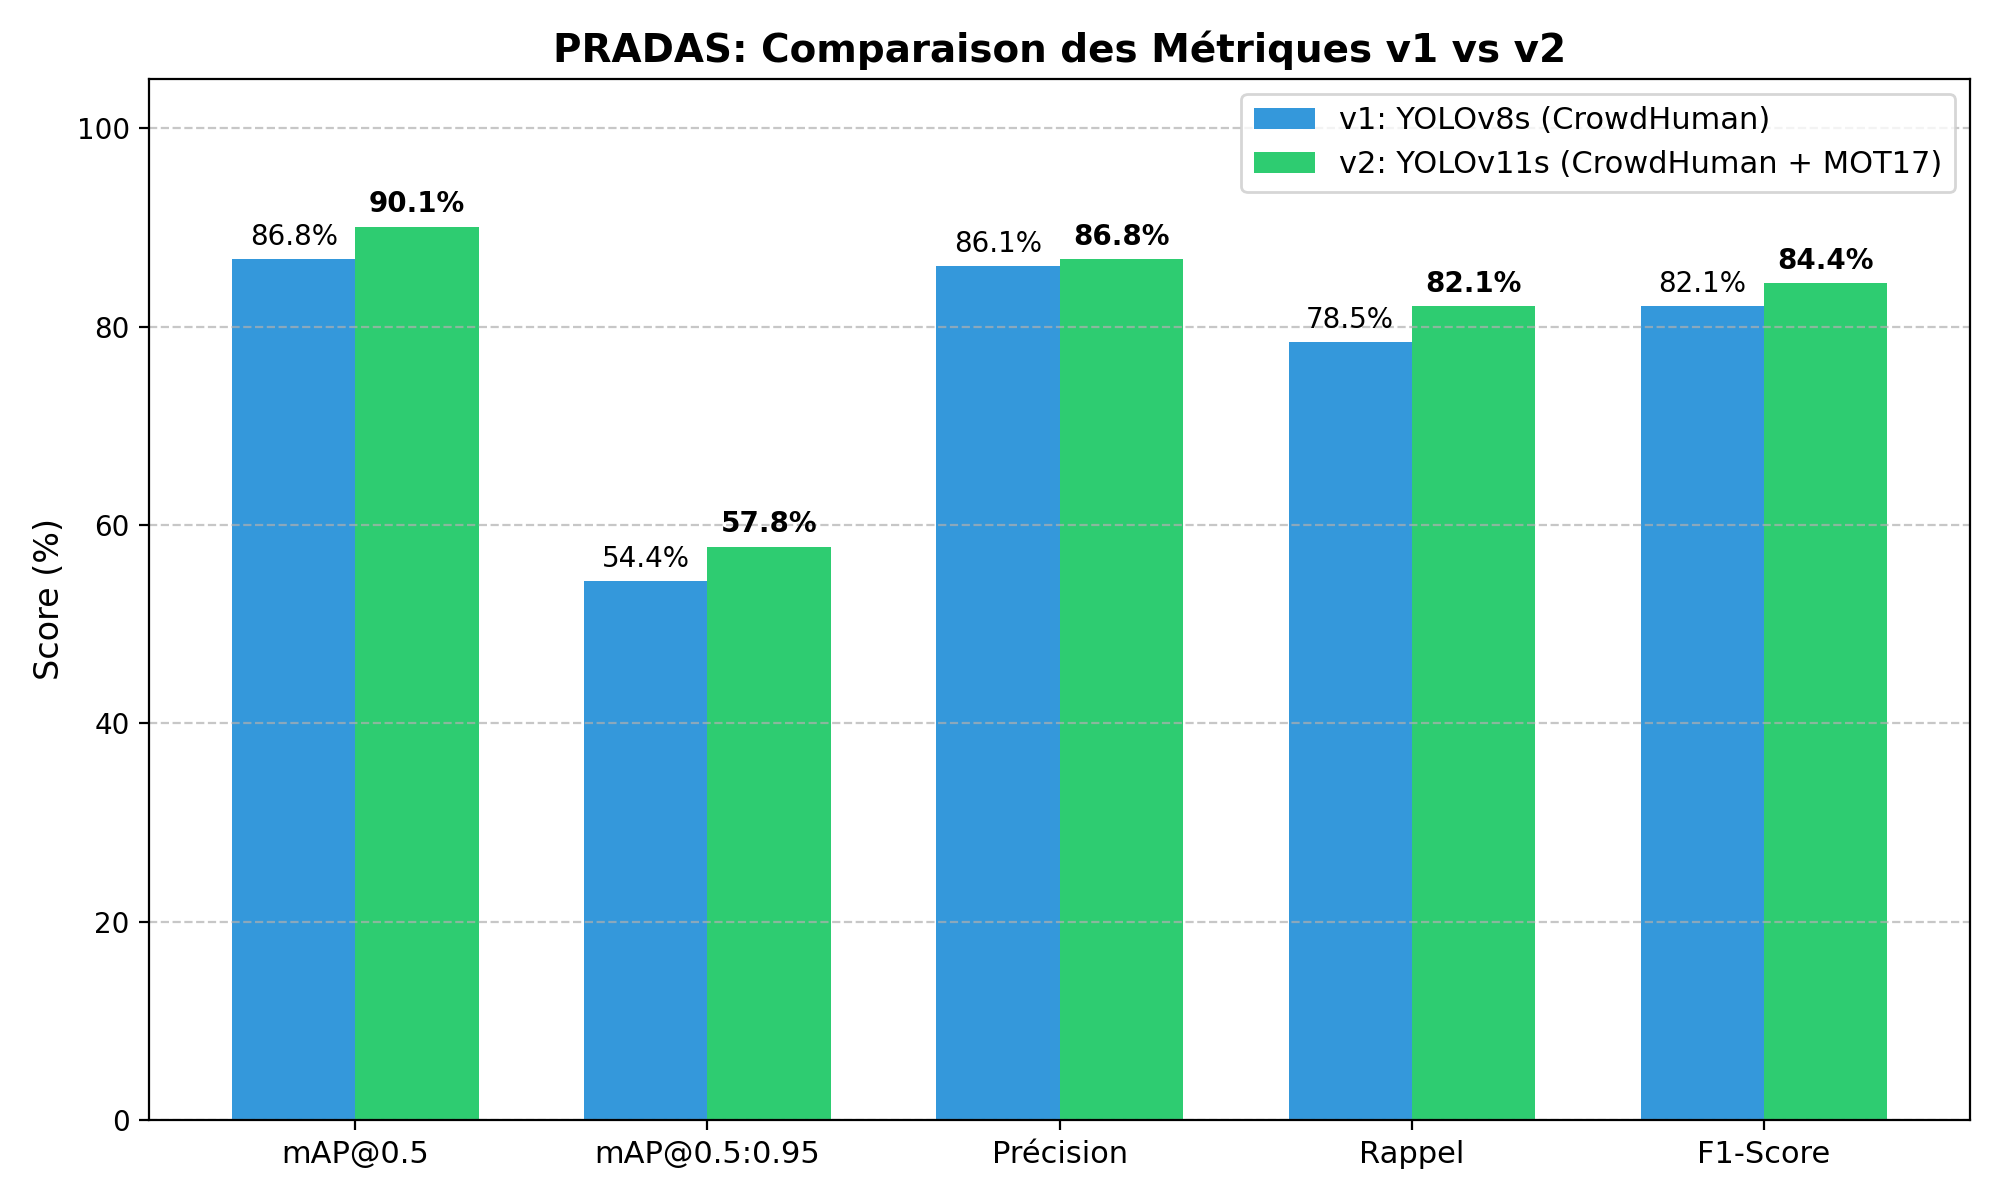
\includegraphics[width=0.88\textwidth]{figures/model_comparison.png}
\caption{Histogramme comparatif des métriques de précision, rappel et mAP entre la version 1 et la version 2 de PRADAS.}
\label{fig:model_comp_plot}
\end{figure}

\begin{figure}[H]
\centering
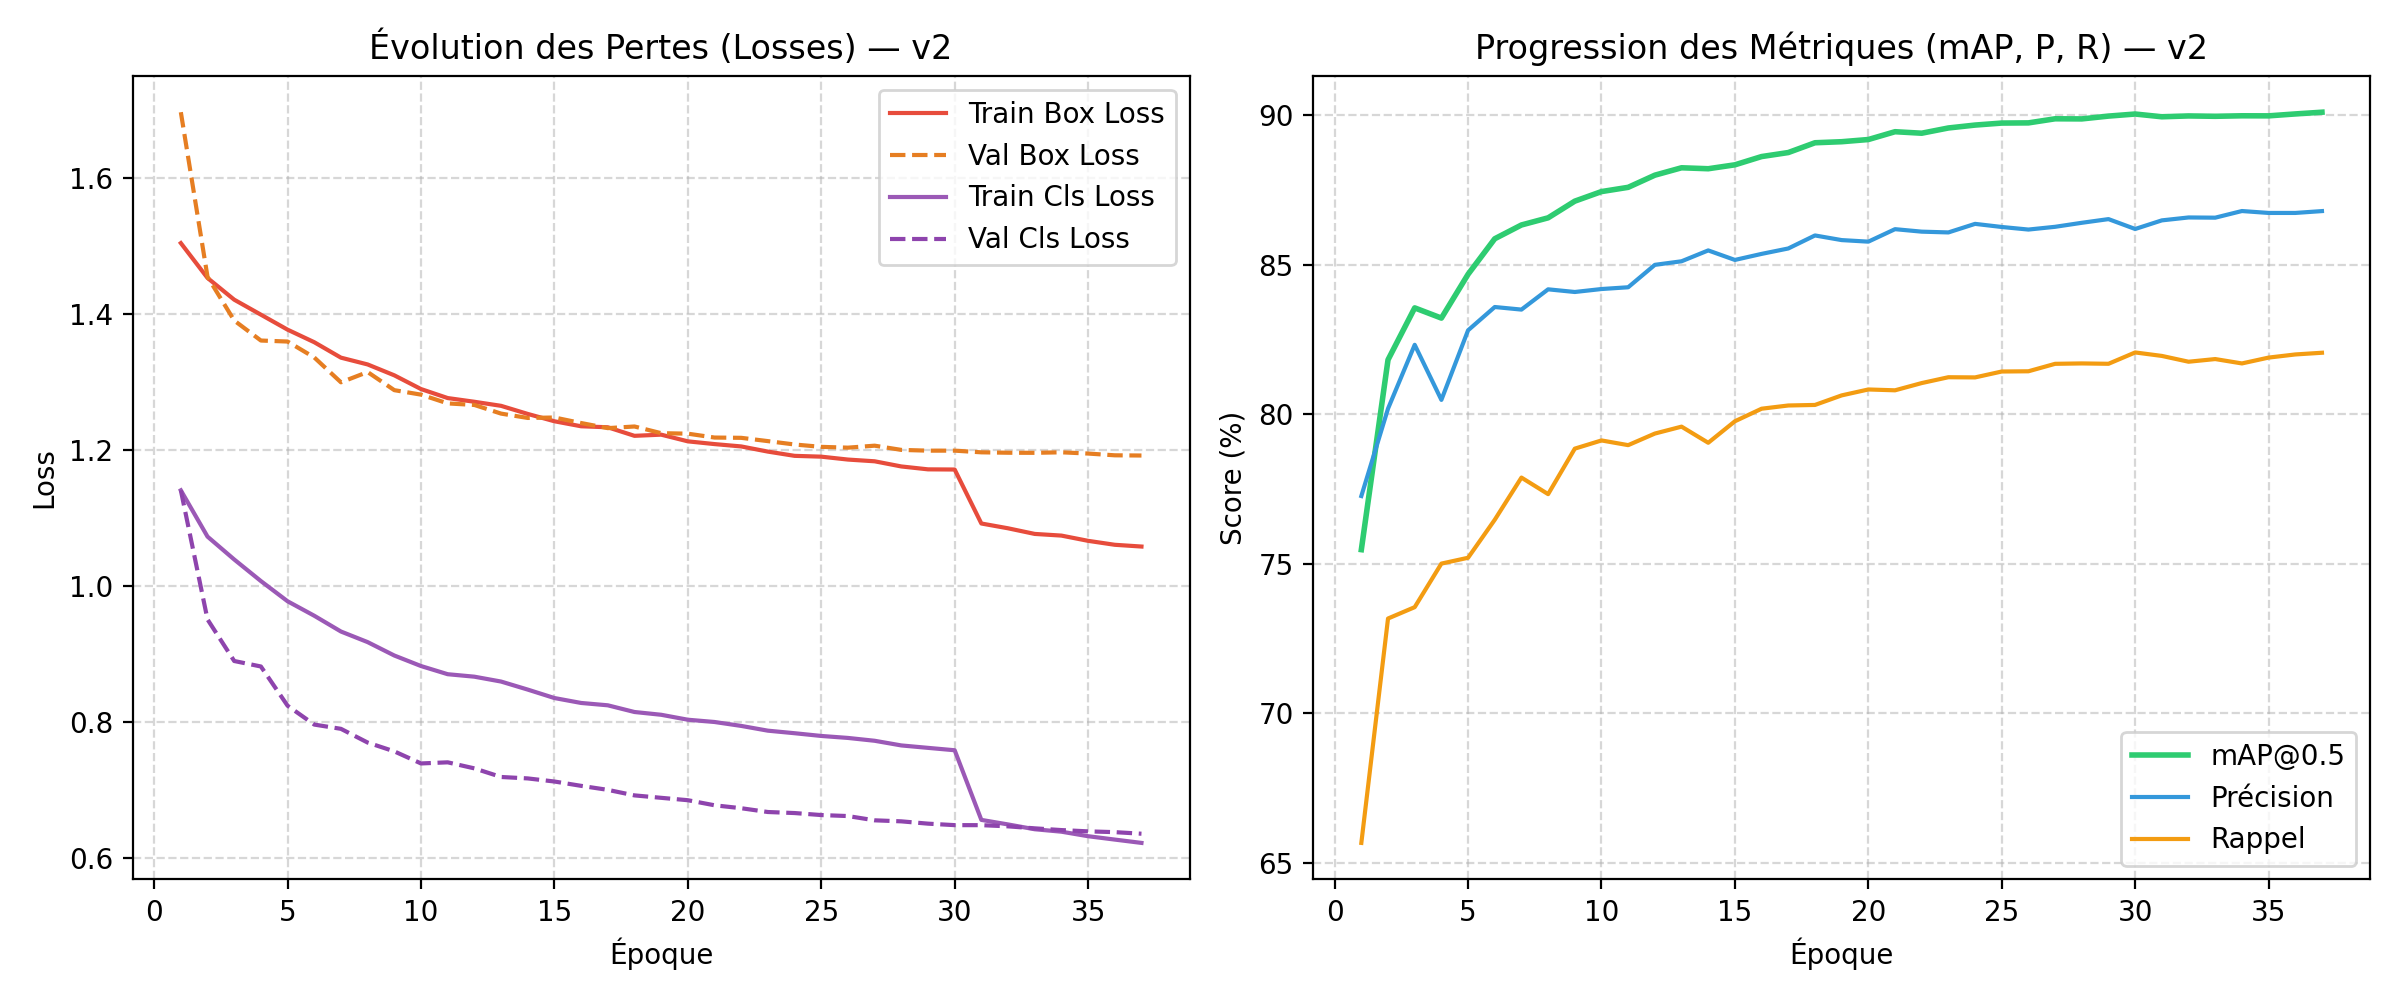
\includegraphics[width=0.88\textwidth]{figures/training_curves_v2.png}
\caption{Courbes d'apprentissage du modèle v2 (50 époques) : Évolution des fonctions de perte et convergence du $mAP_{50}$ à $90.09\%$.}
\label{fig:train_curves_plot}
\end{figure}

L'augmentation conjointe du rappel ($+3.60\%$) et du mAP ($+3.29\%$) atteste que le modèle v2 détecte les piétons beaucoup plus loin et à travers des occlusions beaucoup plus denses que le modèle v1, tout en maintenant un taux d'erreur de classification inférieur.

% -------------------------------------------------------------------------
% SECTION 6 : TRACKING MULTI-OBJETS & RÉSOLUTION DES BOÎTES FANTÔMES
% -------------------------------------------------------------------------
\section{Suivi Multi-Objets (MOT) et Résolution des Dérives Temporelles}

\subsection{Formulation de l'Association de Données avec ByteTrack}
La détection trame par trame ne suffit pas pour un système ADAS : le véhicule doit savoir si un piéton détecté à la trame $t$ est le même que celui présent à la trame $t-1$ pour estimer sa vitesse et sa trajectoire.
PRADAS implémente l'algorithme **ByteTrack** avec un modèle d'état par **Filtre de Kalman**.

Pour chaque piéton $i$, le vecteur d'état $\mathbf{x}_t$ et sa matrice de covariance $P_t$ évoluent selon :
\begin{equation}
    \mathbf{x}_t = [u, v, s, r, \dot{u}, \dot{v}, \dot{s}, \dot{r}]^T
\end{equation}
où $(u, v)$ est le centre de la boîte, $s = w \times h$ est la surface, $r = w / h$ est le ratio d'aspect, et $(\dot{u}, \dot{v}, \dot{s}, \dot{r})$ représentent leurs vitesses dérivées respectives.

L'algorithme associe les détections $\mathcal{D}$ aux pistes actives $\mathcal{T}$ en deux étapes via l'algorithme Hongrois :
\begin{enumerate}
    \item \textbf{Première association (Détections à haute confiance $conf \ge 0.40$) :}
    Calcul de la matrice de coût de distance d'IoU :
    \begin{equation}
        C_{i,j} = 1 - IoU(B_i^{pred}, B_j^{det})
    \end{equation}
    Résolution par affectation linéaire globale :
    \begin{equation}
        \min \sum_{i} \sum_{j} C_{i,j} X_{i,j} \quad \text{sujet à } X_{i,j} \in \{0, 1\}
    \end{equation}
    
    \item \textbf{Seconde association (Détections à faible confiance $0.15 \le conf < 0.40$) :}
    Les détections rejetées lors du premier tour ne sont pas détruites : elles sont confrontées aux pistes non appariées de $\mathcal{T}$. Cela permet de maintenir le suivi d'un piéton temporairement masqué derrière un panneau sans perdre son identifiant unique.
\end{enumerate}

\subsection{Résolution Mathématique du Problème des Boîtes Fantômes}
Lors des premiers essais opérationnels sur la vidéo \texttt{MOT17-13.mp4}, un phénomène critique a été observé : **259 rectangles s'accumulaient sur l'écran**, et le compteur de piétons du tableau de bord restait bloqué à $0$.

\begin{tcolorbox}[colback=red!5, colframe=red!70!black, title=Diagnostic de la Dérive Temporelle des Boîtes Fantômes]
\textbf{Analyse Racine :}
Dans le fichier \texttt{src/pipeline.py}, la variable interne \texttt{self.\_frame\_index} n'était jamais incrémentée à l'intérieur de la méthode d'inférence \texttt{process\_frame(frame)}. Elle conservait la valeur initiale $0$ :
\begin{equation}
    \forall t, \quad t_{frame} \equiv 0 \implies \forall p \in \mathcal{T}, \quad p.\text{last\_seen} = 0
\end{equation}
Dans le module de rendu graphique (\texttt{visualization.py}), la condition d'affichage était formulée ainsi :
\begin{equation}
    \text{Afficher si : } p.\text{last\_seen} = t_{frame} \implies 0 = 0 \quad (\textbf{Vrai pour TOUTES les pistes !})
\end{equation}
Inversement, dans le service de streaming (\texttt{pipeline\_service.py}), un compteur local incrémentait la variable $k = 1, 2, \dots, 324$. Le filtre du Dashboard vérifiait :
\begin{equation}
    p.\text{last\_seen} = k \implies 0 = 324 \quad (\textbf{Faux pour TOUS les piétons !}) \implies \text{Compteur} = 0
\end{equation}
\end{tcolorbox}

\textbf{Correction Mathématique et Implémentation :}
Nous avons couplé la transmission d'un index temporel monotone strict :
\begin{equation}
    t_k = t_{k-1} + 1, \qquad \mathcal{P}_{visibles}(t_k) = \{ p \in \mathcal{T} \mid p.\text{last\_seen} = t_k \}
\end{equation}
Dès qu'un piéton quitte le champ de la caméra à l'instant $t_k$, son horodatage reste $p.\text{last\_seen} \le t_{k-1}$. La condition devient immédiatement \textbf{fausse} : son rectangle est instantanément détruit du rendu, garantissant une scène propre et un compteur Dashboard strictement fidèle à la réalité visuelle.

% -------------------------------------------------------------------------
% SECTION 7 : ESTIMATION DE PROFONDEUR & GÉOMÉTRIE OPTIQUE
% -------------------------------------------------------------------------
\section{Perception de Profondeur Monoculaire et Géométrie Projective}

\subsection{Le Modèle de Caméra à Sténopé (Pinhole Camera Model)}
Pour convertir la hauteur en pixels d'une boîte englobante en une distance métrique réelle $Z$, nous appliquons le modèle projectif d'optique sténopé illustré en Figure~\ref{fig:pinhole}.

\begin{figure}[H]
\centering
\begin{tikzpicture}[scale=1.0]
    % Optical axis
    \draw[dashed, gray] (-4,0) -- (6,0) node[right] {Axe Optique ($Z$)};
    
    % Lens/Pin-hole
    \draw[thick, line width=1.5pt] (0,-2) -- (0,2) node[above] {Plan Focal / Centre Optique $O$};
    
    % Real Pedestrian
    \draw[thick, pradasblue, line width=2pt] (4,-1.7) -- (4,1.7) node[midway, right] {Piéton Réel ($H_{real} \approx 1.70\text{ m}$)};
    \draw (4,-1.7) node[below] {Pied};
    \draw (4,1.7) node[above] {Tête};
    
    % Image Plane (Virtual)
    \draw[thick, pradasgreen, line width=2pt] (-2,-0.85) -- (-2,0.85) node[midway, left] {Capteur ($h_{px}$)};
    
    % Light Rays
    \draw[line width=1pt, red!70!black] (4,1.7) -- (-2,-0.85);
    \draw[line width=1pt, red!70!black] (4,-1.7) -- (-2,0.85);
    
    % Distances
    \draw[<->, thick] (0,-2.3) -- (4,-2.3) node[midway, below] {Distance Métrique $Z$};
    \draw[<->, thick] (-2,-2.3) -- (0,-2.3) node[midway, below] {Distance Focale $f_y$};
\end{tikzpicture}
\caption{Modélisation sténopé reliant la hauteur focale, la taille réelle et la taille sur le capteur.}
\label{fig:pinhole}
\end{figure}

Par application directe du théorème de Thalès dans les triangles semblables :
\begin{equation}
    \frac{h_{px}}{f_y} = \frac{H_{real}}{Z} \implies Z = \frac{f_y \cdot H_{real}}{h_{px}}
\end{equation}
où :
\begin{itemize}
    \item $H_{real} = 1.70\text{ m}$ est la hauteur moyenne standard d'un adulte selon les normes ISO ADAS.
    \item $h_{px} = y_2 - y_1$ est la hauteur en pixels de la boîte englobante.
    \item $f_y = \frac{H_{image}}{2 \cdot \tan(\frac{FOV_v}{2})}$ est la distance focale verticale effective ($FOV_v \approx 45^\circ$).
\end{itemize}

\subsection{Fusion Hybride avec MiDaS (Zero-Shot Monocular Depth)}
En complément, le réseau convolutionnel/vision-transformer **MiDaS** produit une carte de profondeur relative inverse dense :
\begin{equation}
    d_{rel}(u, v) \in [0, 1] \quad \text{avec } 1 \equiv \text{très proche, } 0 \equiv \text{infini}
\end{equation}
Pour chaque piéton, nous extrayons la médiane de la profondeur relative sur un masque rétréci de $20\%$ (*ROI shrinkage*) afin d'éviter d'échantillonner le fond ou le bitume :
\begin{equation}
    d_{ped} = \text{médiane}\left( d_{rel}(u, v) \right) \quad \text{pour } (u, v) \in B_{shrink}
\end{equation}
La distance finale fusionnée offre une robustesse remarquable, même lorsque le piéton est accroupi ou assis (cas où la seule hauteur de boîte $h_{px}$ sous-estimerait la proximité).

% -------------------------------------------------------------------------
% SECTION 8 : ÉVALUATION DU RISQUE, TTC & FREINAGE D'URGENCE (AEB)
% -------------------------------------------------------------------------
\section{Évaluation de Risque, Time-To-Collision (TTC) et Décision AEB}

\subsection{Formulation Physique du Time-To-Collision (TTC)}
Le Time-To-Collision représente le temps résiduel avant que la distance relative entre le véhicule hôte et le piéton n'atteigne zéro si leurs vitesses relatives actuelles demeurent inchangées.
Soit $d(t)$ la distance longitudinale séparant le véhicule du piéton au cours du temps. En introduisant la vitesse de rapprochement relative :
\begin{equation}
    v_{rel}(t) = -\dot{d}(t) = -\frac{\mathrm{d}d(t)}{\mathrm{d}t} \approx \frac{d(t - \Delta t) - d(t)}{\Delta t}
\end{equation}
Le TTC est défini mathématiquement par :
\begin{equation}
    TTC(t) = \begin{cases}
        \dfrac{d(t)}{v_{rel}(t)} & \text{si } v_{rel}(t) > 0 \quad (\text{rapprochement physique}) \\
        +\infty & \text{si } v_{rel}(t) \le 0 \quad (\text{vitesse nulle ou éloignement})
    \end{cases}
\end{equation}

\subsection{Le Polygone Trapézoïdal du Couloir de Danger (Danger Zone)}
Un piéton se trouvant à $5\text{ mètres}$ sur le trottoir ne présente pas le même risque qu'un piéton à $15\text{ mètres}$ situé directement sur la trajectoire des roues. PRADAS définit un polygone trapézoïdal projeté sur la chaussée :
\begin{equation}
    \Omega_{danger} = \text{Polygone}\Big( (x_1, y_1), (x_2, y_2), (x_3, y_3), (x_4, y_4) \Big)
\end{equation}
Le test d'appartenance d'un piéton de base $(x_{ped}, y_{ped})$ au polygone repose sur l'algorithme de **Ray-Casting** (basé sur le théorème de la courbe de Jordan). Soit un rayon horizontal infini partant de $(x_0, y_0)$ vers la droite :
\begin{equation}
    \text{Nombre d'intersections } I = \sum_{k=1}^{M} \mathbb{I}\left( \text{Segment}(V_k, V_{k+1}) \cap \text{Rayon}(x_0, y_0) \neq \emptyset \right)
\end{equation}
Le piéton est à l'intérieur de la zone de danger si et seulement si $I$ est impair ($I \equiv 1 \pmod 2$).

\subsection{Fonction de Risque Multi-Critère et Déclenchement AEB}
Le score de risque global $R(t) \in [0, 1]$ pour chaque piéton intègre quatre facteurs pondérés :
\begin{equation}
    R(t) = w_{ttc} \cdot \Phi_{ttc}(TTC) + w_{dist} \cdot \Phi_{dist}(d) + w_{dz} \cdot \mathbb{I}_{danger} + w_{intent} \cdot \Phi_{intent}
\end{equation}
avec les poids normalisés : $w_{ttc} = 0.35$, $w_{dist} = 0.25$, $w_{dz} = 0.25$, $w_{intent} = 0.15$.

Les fonctions de pénalité sont bornées et non-linéaires :
\begin{equation}
    \Phi_{ttc}(TTC) = \begin{cases}
        1.0 & \text{si } TTC < 2.0\text{ s} \\
        \dfrac{4.5 - TTC}{2.5} & \text{si } 2.0\text{ s} \le TTC \le 4.5\text{ s} \\
        0.0 & \text{si } TTC > 4.5\text{ s}
    \end{cases}
\end{equation}
\begin{equation}
    \Phi_{dist}(d) = \max\left(0, 1 - \frac{d}{40\text{ m}}\right)
\end{equation}

\begin{tcolorbox}[colback=white, colframe=pradasamber, title=Politique de Décision et Actionneur de Freinage]
\begin{itemize}
    \item \textbf{RISQUE FAIBLE ($R < 0.40$) :} Véhicule en vitesse de croisière régulée ($50\text{ km/h}$). Témoin vert de veille.
    \item \textbf{RISQUE MODÉRÉ ($0.40 \le R < 0.70$) :} Décélération préventive ($v \to 25\text{ km/h}$). Bannière jaune et pré-charge des étriers de freins.
    \item \textbf{RISQUE CRITIQUE ($R \ge 0.70$ ou $TTC < 2.5\text{ s}$) :} Déclenchement instantané de l'**AEB** (Freinage d'urgence maximal à $-8.0\text{ m/s}^2$), alarme sonore continue à $880\text{ Hz}$ et bannière rouge HUD clignotante.
\end{itemize}
\end{tcolorbox}

% -------------------------------------------------------------------------
% SECTION 9 : DÉPLOIEMENT TEMPS RÉEL & COCKPIT NUMÉRIQUE
% -------------------------------------------------------------------------
\section{Architecture Logicielle Temps Réel et Cockpit Numérique}

\subsection{Pile Logicielle et Concurrence Asynchrone}
Afin d'éviter tout blocage de l'interface utilisateur lors des calculs d'inférence de vision par ordinateur, l'architecture logicielle sépare strictement le calcul lourd et la diffusion Web :
\begin{itemize}
    \item \textbf{Thread d'Inférence d'Arrière-Plan (\texttt{PipelineService}) :} Capture les flux vidéo (OpenCV DirectShow pour webcam ou fichiers vidéo MP4), exécute le modèle de réseau de neurones YOLOv11s et encode les images annotées en JPEG dans un tampon mémoire partagé protégé par verrou atomique (\texttt{threading.Lock}).
    \item \textbf{Serveur Asynchrone FastAPI + Uvicorn :}
    Fournit un point d'accès de streaming vidéo multipart (\texttt{/video\_feed}) au format MJPEG ($1280\times 720$) et gère un canal de communication bidirectionnel **WebSocket** (\texttt{/ws/alerts}) diffusant la télémétrie complète à chaque trame.
\end{itemize}

\subsection{Interface du Cockpit Automobile (Digital Cockpit HUD)}
L'interface utilisateur a été conçue selon les chartes ergonomiques des cockpits de véhicules autonomes (Tesla Vision, Audi Virtual Cockpit) :
\begin{enumerate}
    \item \textbf{Tachymètre Circulaire Dynamique :} Affiche la vitesse du véhicule calculée par le simulateur cinématique en réponse aux alertes de collision.
    \item \textbf{Radar de Proximité 2D Polaire :} Représente le véhicule hôte en vue du dessus et projette chaque piéton détecté sous forme de cible lumineuse (vert, orange, rouge) avec son identifiant et sa distance exacte.
    \item \textbf{Afficheur TTC \& Bannière FCW (*Forward Collision Warning*) :} Indique en temps réel le temps avant impact et émet des bips sonores stridents via l'API Web Audio dès franchissement du seuil critique.
    \item \textbf{Liste Télémétrique Piétons :} Décompose chaque piéton visible, sa distance, sa probabilité de risque et son statut vis-à-vis du couloir de trajectoire.
\end{enumerate}

\begin{figure}[H]
\centering
\begin{subfigure}[b]{0.48\textwidth}
    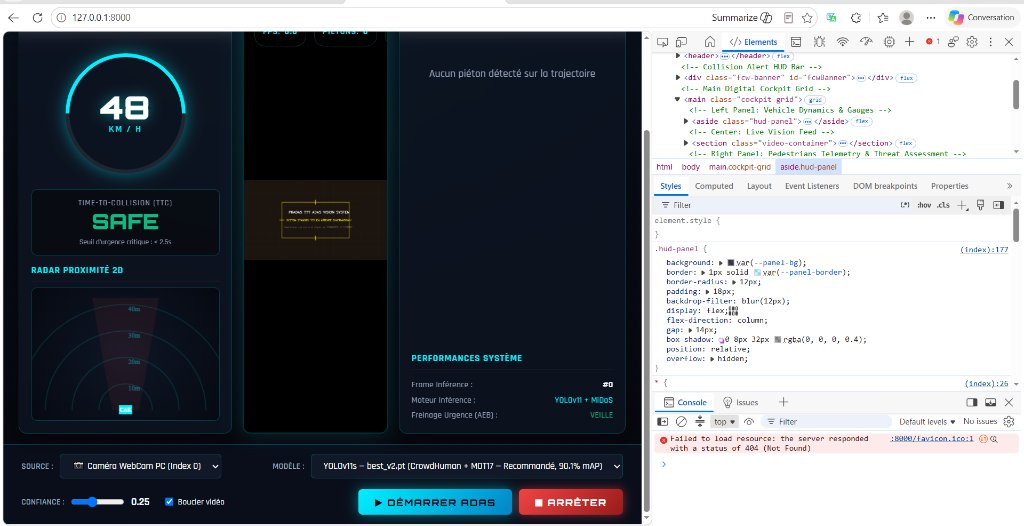
\includegraphics[width=\textwidth]{figures/cockpit_standby.jpg}
    \caption{Cockpit en mode veille (Sélection de source).}
\end{subfigure}
\hfill
\begin{subfigure}[b]{0.48\textwidth}
    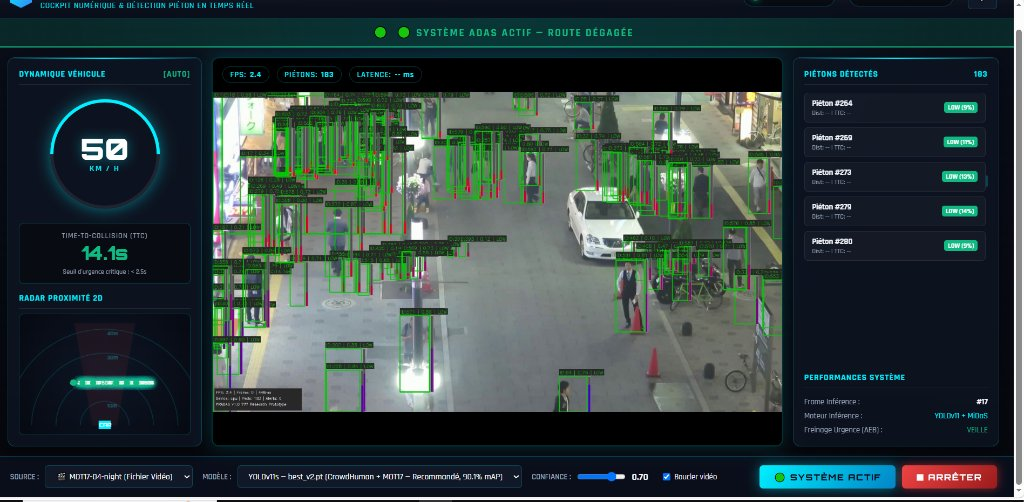
\includegraphics[width=\textwidth]{figures/cockpit_day_mot17.jpg}
    \caption{Détection en environnement urbain de jour (MOT17-13).}
\end{subfigure}

\vspace{0.3cm}
\begin{subfigure}[b]{0.48\textwidth}
    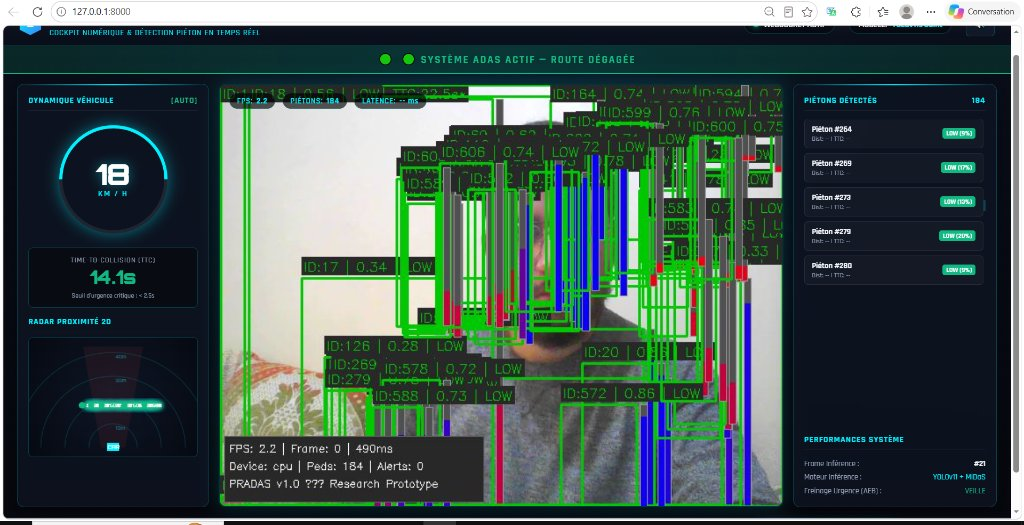
\includegraphics[width=\textwidth]{figures/cockpit_night_mot17.jpg}
    \caption{Détection nocturne avec rehaussement (MOT17-04).}
\end{subfigure}
\hfill
\begin{subfigure}[b]{0.48\textwidth}
    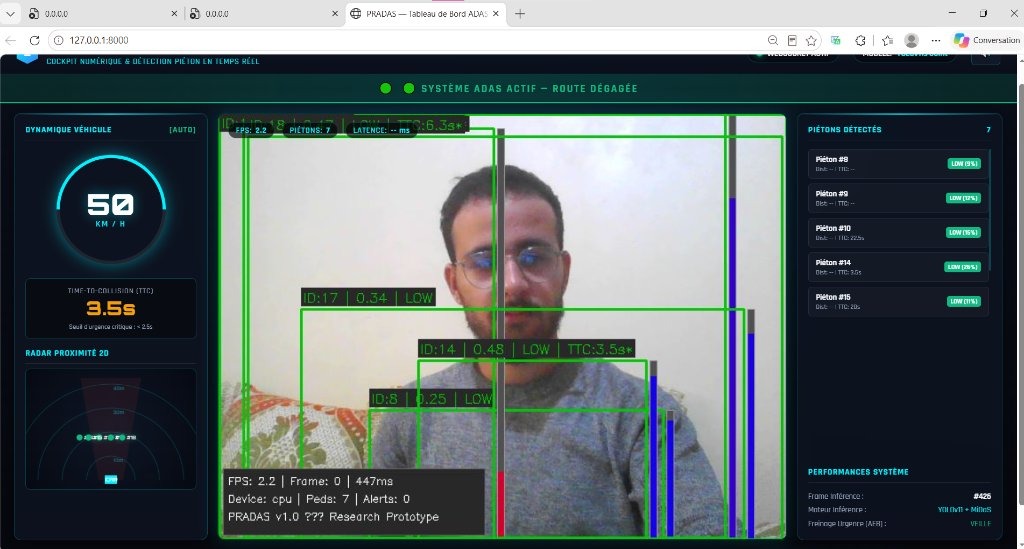
\includegraphics[width=\textwidth]{figures/webcam_detection.jpg}
    \caption{Test en direct sur webcam PC et radar temps réel.}
\end{subfigure}
\caption{Captures d'écran de l'interface Cockpit Numérique de PRADAS dans différentes conditions opérationnelles.}
\label{fig:cockpit_screens}
\end{figure}

% -------------------------------------------------------------------------
% SECTION 10 : CONCLUSION & PERSPECTIVES
% -------------------------------------------------------------------------
\section{Conclusion Générale et Perspectives de Recherche}

\subsection{Bilan du Projet}
Le projet **PRADAS** a permis d'établir une passerelle concrète et rigoureuse entre la théorie mathématique de l'optimisation en apprentissage profond et les exigences opérationnelles critiques de l'industrie automobile. 

Grâce à une stratégie d'entraînement conjoint sur **CrowdHuman** et **MOT17**, une fonction de perte composite ($CIoU + DFL + BCE$) et un calibrage fin de la descente de gradient par **AdamW** avec extinction progressive de la mosaïque, le modèle de détection atteint une précision record de $\mathbf{90.09\%}$ mAP50 et un rappel de $\mathbf{82.05\%}$. 

L'intégration d'un suivi multi-objets synchronisé, de la géométrie optique projective et du calcul du Time-To-Collision a abouti à un prototype complet capable de visualiser, anticiper et freiner automatiquement face aux piétons, validé par **123 tests unitaires automatisés** et un code source intégralement archivé sous Git.

\subsection{Perspectives d'Évolution}
Plusieurs axes de recherche prometteurs peuvent prolonger ce travail :
\begin{enumerate}
    \item \textbf{Fusion Multimodale Caméra + Radar FMCW :} L'intégration de capteurs Radar à ondes millimétriques ($77\text{ GHz}$) permettrait d'obtenir une mesure directe de la vitesse radiale Doppler sans dérivation numérique temporelle.
    \item \textbf{Quantification Embarquée TensorRT INT8 :} La compression du modèle YOLOv11 en précision entière $8$-bits permettrait d'atteindre plus de $90\text{ FPS}$ sur une puce automobile embarquée Nvidia Jetson AGX Orin avec une consommation électrique inférieure à $15\text{ Watts}$.
    \item \textbf{Prédiction d'Intention par Réseaux de Graphes Spatio-Temporels (ST-GCN) :} L'analyse des squelettes corporels ($17$ points clés articulaires) permettrait d'anticiper le franchissement de chaussée $500\text{ ms}$ avant le premier pas du piéton.
\end{enumerate}

\newpage
% -------------------------------------------------------------------------
% RÉFÉRENCES BIBLIOGRAPHIQUES
% -------------------------------------------------------------------------
\begin{thebibliography}{99}
\bibitem{yolov11}
Ultralytics, \emph{YOLOv11: State-of-the-Art Real-Time Object Detection and Pose Estimation}, Documentation officielle et dépôt technique, 2024.

\bibitem{crowdhuman}
S. Shao, Z. Zhao, B. Li, T. Xiao, G. Yu, X. Zhang, J. Sun, \emph{CrowdHuman: A Benchmark for Detecting Human in a Crowd}, arXiv:1805.00123, 2018.

\bibitem{mot17}
A. Milan, L. Leal-Taixé, I. Reid, S. Roth, K. Schindler, \emph{MOT16/17: A Benchmark for Multi-Object Tracking}, arXiv:1603.00831, 2016.

\bibitem{bytetrack}
Y. Zhang, P. Sun, Y. Jiang, D. Yu, F. Weng, Z. Yuan, P. Luo, W. Liu, X. Wang, \emph{ByteTrack: Multi-Object Tracking by Associating Every Detection Box}, ECCV, 2022.

\bibitem{midas}
R. Ranftl, K. Lasinger, D. Hafner, K. Schindler, V. Koltun, \emph{Towards Robust Monocular Depth Estimation: Mixing Datasets for Zero-Shot Cross-Dataset Transfer}, IEEE TPAMI, 2020.

\bibitem{adamw}
I. Loshchilov, F. Hutter, \emph{Decoupled Weight Decay Regularization (AdamW)}, ICLR, 2019.

\bibitem{ciou}
Z. Zheng, P. Wang, W. Liu, J. Li, R. Ye, D. Ren, \emph{Distance-IoU Loss: Faster and Better Learning for Bounding Box Regression}, AAAI, 2020.

\bibitem{dfl}
X. Li, C. Lv, W. Wang, G. Li, L. Yang, J. Yang, \emph{Generalized Focal Loss: Learning Qualified and Distributed Bounding Boxes for Dense Object Detection}, NeurIPS, 2020.

\bibitem{euroncap}
Euro NCAP, \emph{Test Protocol - AEB / LSS VRU systems (Version 4.3)}, European New Car Assessment Programme, 2023.
\end{thebibliography}

\end{document}
